\documentclass[border=3pt]{standalone}
\usepackage{tikz}
\usetikzlibrary{arrows.meta,calc,positioning}
\tikzset{pin/.style={-{Stealth[length=5pt]}},
  blk/.style={draw, thick, minimum width=30mm, minimum height=9mm, font=\sffamily\small, align=center}}
\begin{document}
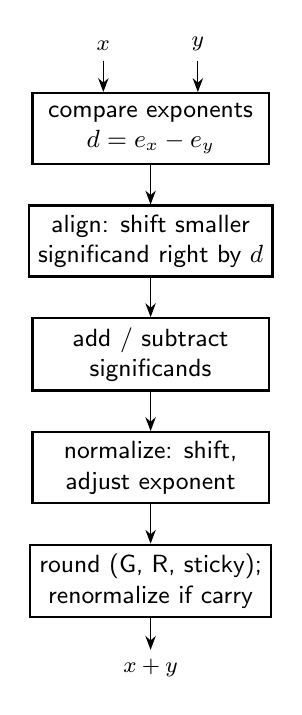
\begin{tikzpicture}[font=\sffamily\small, node distance=5mm]
  \node[blk] (cmp)  at (0,0) {compare exponents\\$d = e_x - e_y$};
  \node[blk, below=of cmp]  (shf) {align: shift smaller\\significand right by $d$};
  \node[blk, below=of shf]  (add) {add / subtract\\significands};
  \node[blk, below=of add]  (nrm) {normalize: shift,\\adjust exponent};
  \node[blk, below=of nrm]  (rnd) {round (G, R, sticky);\\renormalize if carry};
  \draw[pin] ($(cmp.north)+(-6mm,4mm)$) node[above, font=\sffamily\footnotesize]{$x$} -- ($(cmp.north)+(-6mm,0)$);
  \draw[pin] ($(cmp.north)+(6mm,4mm)$) node[above, font=\sffamily\footnotesize]{$y$} -- ($(cmp.north)+(6mm,0)$);
  \draw[pin] (cmp.south) -- (shf.north);
  \draw[pin] (shf.south) -- (add.north);
  \draw[pin] (add.south) -- (nrm.north);
  \draw[pin] (nrm.south) -- (rnd.north);
  \draw[pin] (rnd.south) -- ++(0,-4mm) node[below, font=\sffamily\footnotesize]{$x+y$};
\end{tikzpicture}
\end{document}
